%%% File encoding is ISO-8859-1 (also known as Latin-1)
%%% You can use special characters just like �,� and �

% Custom command fpr the margin notes: \myMarginnote{Your Text}
% Comment on the \lineskiplimit=-\maxdimen:
% See http://tex.stackexchange.com/questions/49072/
% Without it the line spacing of the normal text was changed (ugly).
\newcommand{\myMarginnote}[1]{%
  \marginnote{% needs marginnote package
    \ifthispageodd{\RaggedRight}{\RaggedLeft}% needs ragged2e package
    \color{myColorMainB}%
    \lineskiplimit=-\maxdimen%
    \normalfont\sffamily\scriptsize%
    #1}%
}

% ##############################################
% Start: Header and Footer Customization
% ##############################################
%

% KOMA-Script code for header and footer font
\setkomafont{pageheadfoot}{%
  \normalfont\sffamily\bfseries
}
\setkomafont{pagefoot}{%
  \normalfont\sffamily
}
\setkomafont{pagenumber}{%
  \normalfont\rmfamily
}

% Define width of header
\setheadwidth[0pt]{textwithmarginpar}

% Define with of header line
\setheadsepline{0.4pt}

% Define width of footer
\setfootwidth[0pt]{text}
% Define with of footer line (here: no line)
\setfootsepline[text]{0pt}

% Some calculations
% calc package is needed which is loaded here: 01_Preamble/CommonPackages.tex
% If you want to understand the calculations visit:
% http://en.wikibooks.org/wiki/LaTeX/Page_Layout
\newlength{\myLenghthFootAbstand}
\setlength{\myLenghthFootAbstand}{\paperheight-1in-\topmargin- \headheight-\headsep-\textheight-\footskip}
\newlength{\myLenghthTemp}
\setlength{\myLenghthTemp}{\myLenghthFootAbstand}%+\baselineskip}
\newlength{\cantorSep}
\setlength{\cantorSep}{0.3cm}%
\newcommand\cantorDecoration[1][]{%
  \begin{tikzpicture}[decoration=Cantor set]
    \draw (0.5\cantorSep,0) -- (0.5\cantorSep,\myLenghthTemp);
    \draw decorate{ (0\cantorSep,0) -- (0\cantorSep,\myLenghthTemp) };
    \draw decorate{ decorate{ (-.5\cantorSep,0) -- (-.5\cantorSep,\myLenghthTemp) }};
    \draw decorate{ decorate{ decorate{ (-1\cantorSep,0) -- (-1\cantorSep,\myLenghthTemp) }}};
    \draw decorate{ decorate{ decorate{ decorate{ (-1.5\cantorSep,0) -- (-1.5\cantorSep,\myLenghthTemp) }}}};
    #1
  \end{tikzpicture}%
}

% Define content of header and footer
% Using some scrpage2 commands here. The scrpage2 package is loaded here: 01_Preamble/KOMA-Script-Packages.tex
% Some LaTeX magic...
% Clear all defaults
\clearscrheadfoot
% Header
\ohead{%
  \textcolor{myColorMainA}{\headmark}
}

\patchcmd{\chapter}{\thispagestyle{plain}}{\pagestyle{scrheadings}}{}{}
\patchcmd{\chapter}{\thispagestyle{empty}}{\pagestyle{scrheadings}}{}{}

% Left (even page numbers) footer
\lefoot[%
\PageNumDecor{0,0}{lb}{\rotatebox{180}{\cantorDecoration[\IfInteger{\thepage}{\lifeAnimation{\thepage}}{}]}}%
  \llap{\pagemark~}%
] {%
  \PageNumDecor{0,0}{lb}{\rotatebox{180}{\cantorDecoration[
      \IfInteger{\thepage}{\hourglassAnimation{\thepage}}{}]
    }}%
  \llap{\pagemark~}%
}

% Right (odd page numbers) footer
\rofoot[%
  \PageNumDecor{0.1,0}{rb}{\cantorDecoration[\IfInteger{\thepage}{\lifeAnimation{\thepage}}{\lifeAnimation{1}}]}%
  \rlap{~\pagemark~}%
] {%
  \PageNumDecor{0.1,0}{rb}{\cantorDecoration[\IfInteger{\thepage}{\lifeAnimation{\thepage}}{\lifeAnimation{1}}]}%
  \rlap{~\pagemark~}%
}

\newcommand\PageNumDecor[3]{
  \setlength{\unitlength}{\myLenghthFootAbstand}%
  \begin{picture}(0,0)%
    \put(0,-0.7) {%
      \makebox(#1)[#2]{%
        #3
      } %
      } %
\end{picture}%
}

\newcommand\lifeAnimation[1]{%
  % \pgfmathparse{max(1, floor(#1/2))}
  %\edef\PAGE{\pgfmathresult}

  \begin{scope}[shift={(2,2)},overlay]
    \FPeval\PAGE{max(1,trunc(#1/2:0))}
    \edef\NPAGES{72}
    \FPeval\PAGERES{trunc(\NPAGES * \PAGE / \NPAGES - trunc(\PAGE/\NPAGES:0):0)}

    \ifx\finalversion\undefined
    \node[circle,fill=black] at (0, 3-\PAGERES/60 * 5) {};
    \else
    \node (pic) at (-0.4,5) {\rotatebox{-135}{\includegraphics[page=\PAGERES,scale=0.3]{template/glider/animation/main.pdf}}};
    \fi
%    \useasboundingbox (0,0) rectangle (5cm,5cm);
%    \draw(0,0) rectangle (5cm,5cm);

  \end{scope}
}

\newcommand\hourglassAnimation[1]{%
  \FPeval\PAGE{max(1,trunc(#1/2:0))}
  \begin{scope}[shift={(2,2)},overlay]
    \node (pic) at (0,-\myLenghthTemp) {
      \rotatebox{180}{\resizebox{0.9cm}{\myLenghthTemp}{
          
\includegraphics[page=\PAGE]{template/hourglass/animation/main.pdf}}}};
  \end{scope}
}


%
% #######################
% End: Header and Footer Customization
% #######################


\usepackage[explicit]{titlesec}
\newcommand*\chapterlabel{}
\titleformat{\chapter}
{\gdef\chapterlabel{} \normalfont\sffamily\Huge\bfseries}
{\gdef\chapterlabel{\thechapter\hspace{0.5cm}}}{0pt}
{
  \begin{tikzpicture}[remember picture,overlay]
    \node[yshift=-7cm] at (current page.north west){
      \begin{tikzpicture}[remember picture, overlay]
        \draw[fill=LightGray] (-1,0) rectangle (\paperwidth,7.5cm);
        %
        \ifx\finalversion\undefined
        \else
        \node[opacity=0.05] (gofl) at (0.5\paperwidth,5.25cm) {
          \ifthenelse{\equal{\LifeChapter}{}}{}{
            
\includegraphics[width=\paperwidth]{figures/myelin_bw3.eps}
          }
        };
        %
        \node[opacity=0.1, align=center, text width=0.9\linewidth, font=\ttfamily\footnotesize,below=0cm of gofl](bf) {
          \ifthenelse{\equal{\BrainFuckChapter}{}}{}{
            \begin{center}
              \color{DarkGray}
              \BrainFuckChapter{}
            \end{center}
          }
        };
        \fi
        %
        \node[xshift=0.5\paperwidth,anchor=east, rectangle, rounded corners=20pt, inner sep=11pt,fill=black] at (0.5\linewidth,0)
        {\color{white}\Huge\bfseries\chapterlabel#1};
        %
      \end{tikzpicture}
    };
  \end{tikzpicture}
}
\titlespacing*{\chapter}{0pt}{7.5cm}{-60pt}


\usepackage{xparse}
\NewDocumentCommand\chapterWHeading{s m}{
  \chapter*{#2}
  \markboth{#2}{#2}
}

%%% Local Variables:
%%% mode: latex
%%% TeX-master: "../main"
%%% End:
